\chapter{Arbejdsmetoden}
\label{arbejdsmetoden}

\section{Objekt Orienteret Analyse & Design}


\section{Den evolutionære- kontra den konstruktive arbejdsmetode}

Den evolutionære arbejdsmetode er en metode, som er velegnet i en udviklingsproces, af et system, hvor der interageres med brugerer/informanter. 
Metoden tager udgangspunkt i iterationer ved, at et forløb deles op i en række faser, som hver gennemgår samtlige af projektes dele. 
Et systemudviklingsprojekt kunne eksempelvis være delt op i følgende punkter: analyse, design, programmering, aftestning og afprøvning, som præsenteret i \figref{fig:evolutionaeremetode}. Figuren er, ligesom \figref{fig:konstruktivemetode} og \figref{fig:blandingsmetode}, taget fra slides, fra Objekt Orienteret Analyse & Design \cite{ooadslide}, og tilpasset til vores egen projektforløb.
For hver fase vil der blive tilføjet, fjernet eller på anden vis redigeret i indholdet fra delene, så de hele tiden er opdateret i forhold til det problem, der skal løses. 
Metoden er specielt anvendelig i forhold til udviklingsprocesser, hvor problemet, som skal løses, ikke er veldefineret, eller ændres undervejs i forløbet. 
Som et eksempel på dette kan vi nævne vores egne erfaringer. I løbet af projektet havde vi formuleret nogle midlertidige problemformuleringe, men den endelige problemformulering blev fastlagt i slutningen af projektforløbet, da vi først her var færdige med at fortolke og revidere vores forståelse af problemet.
Her kan udviklingsprocesen, ved hjælp af den evolutionære metode, nemt ændres og dirigeres henimod det rette problem igen.

\begin{figure}[ht]
	\centering
	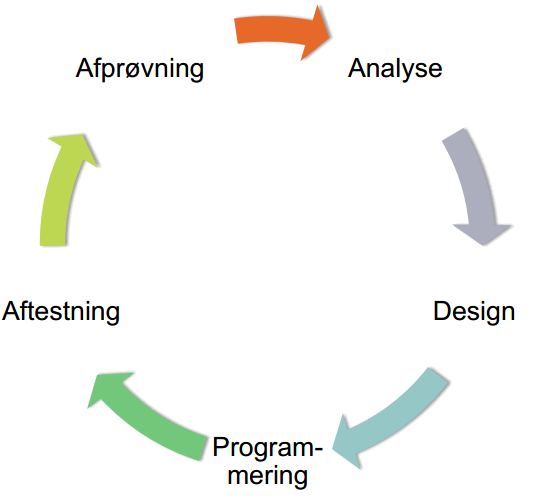
\includegraphics[scale=0.5]{billeder/evolutionaeremetode.png}
	\capt{Figuren illustrerer en fase i den evolutionære arbejdsmetode. En enkelt fase i udviklingsforløbet gennemgår samtlige dele af projektet.}
	\label{fig:evolutionaeremetode}
  \end{figure}

Modsat findes den konstruktive arbejdsmetode (også kaldet vandfaldsmetoden), som har en liniær tilgang til udviklingsprocessen. Den konstruktive arbejdsmetode er også delt op i faser, men hver fase er modsat i den evolutionære metode, fokuseret henimod en specifik projektdel (se \figref{fig:konstruktivemetode}). Typisk vil et systemudviklingsforløb med udgangspunkt i den kontruktive arbejdsmetode starte ud med en analyse. Når analysen er færdig, påbegyndes design, og derefter programmering osv. Metoden bruges ofte i systemudviklingsprocesser, hvor det problem, der arbejdes ud fra, er veldefineret og klart. Det er grundet, at metoden ikke, på samme måde som den evolutionære arbejdsmetode, er dynamisk i forhold til, hvis problemet ændrer sig undervejs i forløbet.

\begin{figure}[ht]
	\centering
	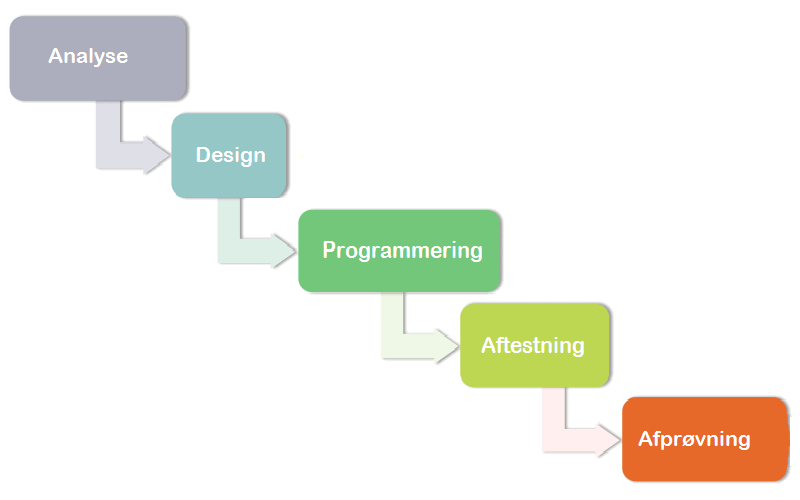
\includegraphics[scale=0.5]{billeder/konstruktivemetode.png}
  	\capt{Figuren illustrerer den konstruktive arbejdsmetode.}
  	\label{fig:konstruktivemetode}
\end{figure}

Vi har kort beskrevet den evolutionære og den konstruktive arbejdsmetode. Desuden har vi beskrevet, at den evolutionære arbejdsmetode er mere fleksibel i forhold til den konstruktive arbejdmetode, når det problem, der skal løses, ændrer sig. Men hvilke andre fordele og ulember er der, ved at vælge den ene arbejdsmetode frem for den anden? Det kommer meget an på situationen.

En forskel mellem de to metoder er bl.a. deres måde at interagere med bruger/informanter på. Mens der foregår et tæt samarbejde med informanter i den evolutionære arbejdsmetode, hvor der anvendes prototyper; har informanterne en mere passiv rolle i den konstruktive metode, hvor de blot godkender beslutninger, og fungerer som ressourcer til informantion. Alt efter hvilke brugere/informanter man arbejder sammen med i sit projekt, vil den ene arbejdsmetode være at foretrække frem for den anden. En anden forskel mellem de to metoder er deres tilgang til det endelig produkt/system. Den konstruktive arbejdsmetode har en meget stringent og langsigtet tidsplan, og man er ikke i tvivl om, hvornår produktet/systemet er færdigt. I en systemudviklingsproces med den evolutionære arbejdsmetode kan det modsat være svært at vurdere,  hvornår systemet er færdigt. Det vil altid være muligt at gå igennem endnu en iteration, og lave nye tilføjelser og redigeringer.

\begin{figure}[ht]
	\centering
	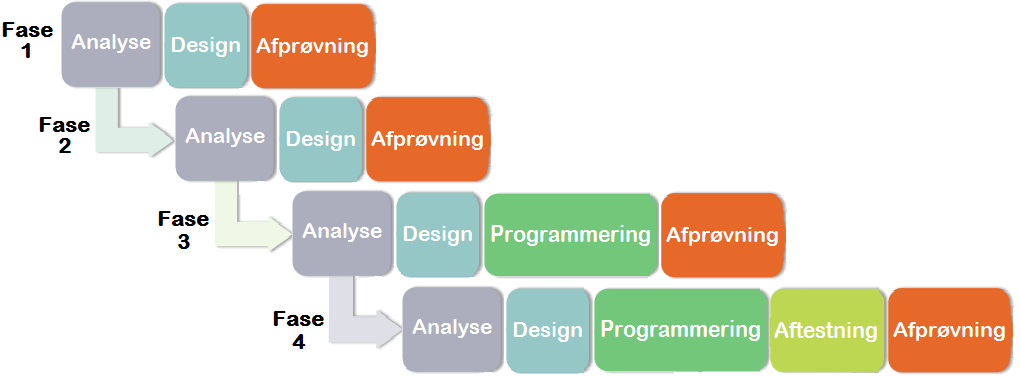
\includegraphics[scale=0.5]{billeder/blandingsmetode.png}
  	\capt{Figuren illustrerer gruppens arbejdsmetode, som har været en blanding mellem den evolutionære og konstruktive arbejdsmetode.}
  	\label{fig:blandingsmetode}
\end{figure}

Der er altså store forskelle på de to arbejdsmetodes tilgang til en systemudviklingsproces, og det er derfor op til situationen, hvilken der vil fungere bedst. Det er dog væsentligt at nævne, at det næsten aldrig vil være muligt, i en udviklingsproces, udelukkende at arbejde ud fra den ene arbejdsmetode. Som regel vil elementer fra begge arbejdsmetoder, blive implementeret, men én vil være dominerende. I vores projektforløb, anvendte vi også elementer fra begge metoder, men udgangspunktet var den evolutionære arbejdsmetode. Dette var grundet, at problemet som vi fokuserede på, ikke var fuldkommen klart i den initierende del af forløbet. Vi havde kurser, sideløbende med projektet, som gjorde at vi ikke kunne komme igennem hver eneste projektdel, da vi først skulle introduceres for nogle begreber, i vores kurser omhandlende systemudvikling \cite{ooad} og designing interactive systems \cite{deb}. Vores arbejdsmetode, er illustreret i \figref{fig:blandingsmetode}. Vi delte processen op i 4 faser, hvor vi i de to første faser, udelukkende arbejdede med analyse- og designdelen, samt afprøvening ved hjælp af protoyper. Først i tredje fase begyndte vi at programmere og teste programmet, og det samme gjorde vi i fase fire. Den måde vores forløb var iterativt på, var ved at vi i hver fase gik tilbage, og tilføjede, redigerede eller slettede noget i de dele, som vi havde gennemgået i den foregående fase.

Til fremtidige projekter, ville den evolutionære arbejdsmetode bestemt være en metode gruppen ville overveje at bruge igen i lignende forløb. Den tætte interaktion med brugere/informanter, mener vi er essentiel i systemudvikling, fordi det i sidste ende er brugerne som skal bruge det færdige system, og derfor er det vigtigt at systemet opfylder brugernes behov. Derudover er det faktum, at metoden er så fleksibel som den er, med til at gøre den mere anvendelig til projektforløb, end den konstruktive arbejdsmetode. Dette er grundet, at der sideløbende med projektet, ofte er kurser, som introducerer begreber, der skal implementeres til projektet, hvilket er nemmere med den evolutionære metode. Dette mener vi tilgengæld også er metodens største svaghed, da de konstante tilføjelser og redigeringer, også kræver en revidering af rapporten. Det vil sige, at selv i et projektforløbs afsluttende fase, kan der stadig blive revideret i rapportens analysedel, designdel osv., og det giver en stor udfordring i forhold til at bibeholde en naturlig sammenhæng i rapporten. 


%% Hvordan kunne det være blevet gjort bedre i fremtidige projekter?

%% DONE:
%% konstruktive metode
%% fordele og ulember
%% Hvad har vi anvendt?
